\documentclass[11pt]{article}
\usepackage[a4paper,margin=1in]{geometry}
\usepackage{amsmath,amssymb,amsthm,mathtools}
\usepackage[expansion=false]{microtype}
\usepackage{graphicx,booktabs,array}
\usepackage[font=small,labelfont=bf]{caption}
\usepackage[dvipsnames]{xcolor}
\usepackage{enumitem}
\usepackage[hidelinks,pdfusetitle]{hyperref}
\usepackage[nameinlink,capitalise]{cleveref}
\setlist{nosep,leftmargin=1.5em}
\newtheorem{theorem}{Theorem}
\newtheorem{lemma}[theorem]{Lemma}
\newtheorem{proposition}[theorem]{Proposition}
\newtheorem{corollary}[theorem]{Corollary}
\theoremstyle{definition}\newtheorem{definition}[theorem]{Definition}
\theoremstyle{remark}\newtheorem{remark}[theorem]{Remark}
\newenvironment{mainresult}[1]{\par\medskip\noindent\textbf{#1}\ \itshape\ignorespaces}{\par\medskip}
\newcommand{\R}{\mathbb R}\newcommand{\C}{\mathbb C}\newcommand{\N}{\mathbb N}
\newcommand{\dd}{\,\mathrm d}\newcommand{\e}{\mathrm e}
\newcommand{\Num}{\mathrm{Num}}\newcommand{\Den}{\mathrm{Den}}
\renewcommand{\Re}{\operatorname{Re}}\renewcommand{\Im}{\operatorname{Im}}
\setlength{\parskip}{0.35em}
\AtBeginDocument{\sloppy}
\urlstyle{same}
\hypersetup{pdftitle={The Reversible Half and the Third Body: Pairs and Triads in Measurement Records and the Three-Body Problem},pdfauthor={Abhijit Singh}}
\title{\textbf{The Reversible Half and the Third Body: Pairs and Triads in Measurement Records and the Three-Body Problem}}
\author{Abhijit Singh}
\date{25 September 2026}
\begin{document}
\maketitle
\begin{abstract}
Time reversal is an involution: it splits every quantity into a part it keeps and a part it reverses. We determine what the reversed part carries in two settings, the classical records written by sequential quantum measurement and three equal masses under gravity. For a record chain $C$ with stationary law $\pi$, time reversal $\tilde C$ and reversible half $S=\frac12(C+\tilde C)$, we prove that the entropy the record forgoes by being directed is a $\pi$-average of Jensen--Shannon divergences between its forward and time-reversed transition laws, and that $0\le h(S)-h(C)\le\frac14\mathrm{EP}$, where EP is the entropy production, with equality to leading order as $C\to S$. The bound rests on the pointwise inequality $\mathrm{JSD}\le\frac18\times$(Jeffreys divergence). For alternating sharp measurement of a singlet with $n\ge3$ settings we solve the record exactly: the stationary record is reversible, and a record of length $L$ carries total irreversibility $\frac c2(1-d^{L-2})\log_2\frac{1+c}{1-c}$ bits, $c=\cos\frac\pi n$, $d=\cos\frac{2\pi}n$, whose limit $c\,\mathrm{artanh}(c)$ nats is the Jeffreys divergence of the seed pair law from the stationary one; a separable preparation writes the identical record. A processed four-outcome instrument reconstructed from tomography writes its arrow continuously, at $\mathrm{EP}=0.00686044$ bits per use, with $h(S)-h(C)$ at $99.86\%$ of $\mathrm{EP}/4$. The rotating field of three-phase currents carries the same involution: time reversal transposes its lagged correlation matrix $K(\tau)$, whose symmetric half carries the magnitude $|I_+|^2+|I_-|^2$ and whose antisymmetric half carries the signed swept area $\frac{9\pi}4(|I_+|^2-|I_-|^2)$.

For three equal masses we prove that every collinear instant with one body at the midpoint is the triad $(-s,0,s)$ about the centre of mass, that three bodies on one curve at thirds of the period carry no harmonic divisible by three, that the time-reversal symmetry of the figure-eight makes its angular momentum vanish harmonic by harmonic, as a balance of counter-rotating pairs, and that the equal-mass Lagrange triangle grows at exactly $\omega/\sqrt2$. The figure-eight has period $T=6.3259140121$; it is a choreography to $1.3\times10^{-8}$ from the published initial data and to $4.1\times10^{-12}$ from refined data that close the orbit to $9.6\times10^{-13}$; it holds the triad six times per period, at $kT/6$ to $5.5\times10^{-9}$, with each body at the zero twice; and it keeps its shape within $3.2\times10^{-6}$ over $50$ periods after a $10^{-6}$ kick, while the Lagrange triangle grows at $0.702194$ against the exact $\omega/\sqrt2=0.702331$. A fourth body of mass $\varepsilon$ at distance $D$ outside the Mardling--Aarseth boundary lends the triad a spin and takes it back every half outer orbit, deforming it by $\delta_{\max}\simeq\sqrt3\langle\Delta I\rangle\varepsilon D^{-3/2}=2.84\,\varepsilon D^{-3/2}$; the triad keeps its shape to $10^{-2}$ for $\varepsilon/D^3\le10^{-4}$ and loses it for $\varepsilon/D^3\ge3.7\times10^{-4}$, and inside the boundary the fourth body is expelled. The proofs use convexity, Fourier series on the cube roots of unity and the symmetries of Newton's equations; the orbits are integrated by an eighth-order Runge--Kutta method at tolerances $10^{-12}$ to $10^{-13}$.
\end{abstract}

\section{Introduction}\label{sec:intro}
A measurement record is written by an observer, and time reversal pairs every record with its reverse. Three bodies under gravity, which couples every pair of bodies with the same sign, carry a time reversal of their own. In both settings the involution splits every quantity into an even half and an odd half. This paper determines what the odd half carries, how large it can be, and where it vanishes.

\paragraph{Records.} Sequential use of a quantum instrument, an outcome map together with its conditional successor state, produces a classical record $X_0,X_1,\dots$ \cite{Kraus,Singh}. Much is known about what such records certify (Bell nonlocality \cite{Bell}, contextuality \cite{KS}, randomness) and what their erasure costs \cite{Landauer,ReebWolf,delRio}. We ask whether the record \emph{has a direction}: whether the statistics of the reversed sequence differ from those of the sequence itself, by how much, and what the difference costs in entropy. The natural measure is the entropy production of the record process \cite{Schnakenberg,Gaspard,GaspardErr}, the rate at which forward and reversed records become distinguishable. When the record variables are a coarse description of the process that writes them, this statistical irreversibility bounds the physical dissipation from below and need not equal it \cite{KPV,RoldanParrondo}; the corresponding statistic for continuous quantum measurement was studied by Dressel et al.\ \cite{Dressel}. The reversible chain $S=\frac12(C+\tilde C)$ is Fill's additive reversiblization \cite{Fill}.

\paragraph{Three bodies.} The prior results this paper builds on form a sequence (\cref{tab:prior}). Gascheau and Routh found when the rotating equilateral triangle of three masses is linearly stable \cite{Gascheau,Routh}. The figure-eight was found numerically by Moore \cite{Moore}. Chenciner and Montgomery proved its existence and gave Sim\'o's initial data \cite{CM}: $x_1=-x_2=(0.97000436,-0.24308753)$, $x_3=0$, $\dot x_3=-2\dot x_1=-2\dot x_2=(-0.93240737,-0.86473146)$, with unit masses, $G=1$ and period $6.32591398$. Sim\'o studied its dynamics numerically \cite{Simo}. Roberts proved its linear stability with rigorous numerical estimates: its nontrivial characteristic multipliers are distinct and lie on the unit circle \cite{Roberts}. Mardling and Aarseth gave the stability boundary of hierarchical triples used in \cref{sec:fourth} \cite{MA}. At $t=0$ the figure-eight's configuration is $(s,-s,0)$, the triad itself.

\begin{table}[!htb]\centering\small
\begin{tabular}{@{}l>{\raggedright\arraybackslash}p{4.2cm}>{\raggedright\arraybackslash}p{8.4cm}@{}}\toprule
year & authors & result\\\midrule
1843, 1874 & Gascheau; Routh \cite{Gascheau,Routh} & the Lagrange triangle is linearly stable iff $27\sum_{i<j}m_im_j<(\sum_im_i)^2$\\
1993 & Moore \cite{Moore} & the figure-eight found numerically\\
2000 & Chenciner, Montgomery \cite{CM} & existence of the figure-eight; Sim\'o's initial data\\
2001 & Mardling, Aarseth \cite{MA} & stability criterion for hierarchical triples\\
2002 & Sim\'o \cite{Simo} & dynamical properties of the figure-eight\\
2007 & Roberts \cite{Roberts} & linear stability of the figure-eight\\\bottomrule
\end{tabular}
\caption{Prior results on three bodies used in this paper.}\label{tab:prior}
\end{table}

\paragraph{Companion papers.} The singlet of \cref{sec:singlet} is the fourth state of the decomposition $\frac12\otimes\frac12=1\oplus0$, whose triplet is the triad, and the identity $1+u+u^2=0$ that removes the harmonics divisible by three in Theorem~1.4(b) is the identity that makes a probe qubit coupled to a maximally mixed spin-1 decohere completely at $\frac13$ and $\frac23$ of its revival period \cite{SQuant}. The restricted problem, where one of three masses vanishes, is treated in \cite{SPlanet}: there each giant planet's Hill sphere opens through two throats at $L_1$ and $L_2$, a pair about the planet, and the triangular points are the Lagrange triangle of \cref{sec:exact} with one vanishing mass, stable by the Gascheau--Routh criterion \cite{Gascheau,Routh}; the Trojans of the four giant planets and the fourth bodies that deplete them are treated there as well.

\subsection{Main results}\label{sec:main}
Let $C$ be a column-stochastic matrix, $C_{ij}=\Pr(X_{t+1}=i\mid X_t=j)$, irreducible with stationary law $\pi$, stationary pair law $J_{ij}=\pi_jC_{ij}$ and time reversal $\tilde C=D_\pi C^{\mathsf T}D_\pi^{-1}$, $D_\pi=\operatorname{diag}(\pi)$. Write $h$ for the entropy rate of a chain and $\mathrm{EP}(C)=D(J\,\|\,J^{\mathsf T})$ for the entropy production of the record (\cref{def:ep}).

\begin{mainresult}{Theorem 1.1 (the reversible half).}
Assume $J_{ij}>0\iff J_{ji}>0$, and write $C=S+A$ with $S=\frac12(C+\tilde C)$ and $A=\frac12(C-\tilde C)$. Then:
\begin{enumerate}
\item $S$ is column-stochastic with stationary law $\pi$ and satisfies detailed balance; $A$ has zero column sums and $AD_\pi=\frac12(J-J^{\mathsf T})$ is antisymmetric.
\item $h(S)-h(C)=\sum_j\pi_j\,\mathrm{JSD}(C_{\cdot j},\tilde C_{\cdot j})\ge0$, where JSD is the Jensen--Shannon divergence.
\item $\mathrm{EP}(C)=\sum_j\pi_jD(C_{\cdot j}\|\tilde C_{\cdot j})=\sum_j\pi_jD(\tilde C_{\cdot j}\|C_{\cdot j})$, and
\[
0\ \le\ h(S)-h(C)\ \le\ \tfrac14\,\mathrm{EP}(C),
\]
with equality in either inequality iff $A=0$; as $A\to0$ at fixed $S$, $h(S)-h(C)=\frac14\mathrm{EP}(C)\,(1+O(\|A\|^2))$.
\end{enumerate}
\end{mainresult}

\begin{mainresult}{Theorem 1.2 (the arrow of the singlet walk).}
Let $n\ge3$, $\vartheta=\pi/n$, $c=\cos\vartheta$, $d=\cos2\vartheta$ and $O(\theta)=\cos\theta\,\sigma_z+\sin\theta\,\sigma_x$. Starting from the singlet $|\Psi^-\rangle=(|01\rangle-|10\rangle)/\sqrt2$, measure $O(k\vartheta)$ sharply at step $k$ on Alice for even $k$ and on Bob for odd $k$, recording $X_k\in\{\pm1\}$. Then $\Pr(X_0=a)=\frac12$, $\Pr(X_1=b\mid X_0=a)=\frac{1-abc}2$ and $\Pr(X_k=x\mid X_{<k})=\frac{1+xX_{k-2}d}2$ for $k\ge2$, and:
\begin{enumerate}[label=(\alph*)]
\item the stationary record, with $(X_0,X_1)$ uniform and the same distance-two transitions, is reversible: every stationary block law is invariant under reversal;
\item for every record length $L\ge2$ and every sequence, $\log\frac{P_\to(x_0,\dots,x_{L-1})}{P_\to(x_{L-1},\dots,x_0)}=\log\frac{1-x_0x_1c}{1-x_{L-1}x_{L-2}c}$, and the total irreversibility of the record is
\[
\mathcal D_L:=D\bigl(P_\to^{(L)}\,\|\,P_\leftarrow^{(L)}\bigr)=\frac c2\bigl(1-d^{L-2}\bigr)\log_2\frac{1+c}{1-c}\ \text{bits}\ \xrightarrow[L\to\infty]{}\ \frac{c\,\mathrm{artanh}(c)}{\ln2}\ \text{bits};
\]
\item the limit equals the Jeffreys divergence between the law $\frac14(1-x_0x_1c)$ of $(X_0,X_1)$ and the uniform law of an adjacent pair in the stationary record;
\item the separable state $\frac12(|0\rangle\langle0|\otimes|1\rangle\langle1|+|1\rangle\langle1|\otimes|0\rangle\langle0|)$ writes the identical record law.
\end{enumerate}
\end{mainresult}

\begin{mainresult}{Theorem 1.3 (the rotating field).}
Let three coils at angles $0,\pm120^\circ$ carry the currents $i_k(t)=\Re(I_k\e^{i\omega t})$, $k\in\{a,b,c\}$, and let $B(t)=i_a(t)+u\,i_b(t)+u^{-1}i_c(t)$ be their field, $u=\e^{2\pi i/3}$. With $I_\pm=\frac13(I_a+u^{\pm1}I_b+u^{\mp1}I_c)$ and $I_0=\frac13(I_a+I_b+I_c)$,
\[
B(t)=\alpha_+\e^{i\omega t}+\alpha_-\e^{-i\omega t},\qquad \alpha_+=\tfrac32I_+,\quad \alpha_-=\tfrac32\overline{I_-}.
\]
\begin{enumerate}
\item The zero-sequence part $I_0$ does not contribute. Reversing the phase order ($b\leftrightarrow c$) exchanges $I_+$ and $I_-$, and reversing time ($t\mapsto-t$) exchanges the magnitudes of the forward and backward components.
\item The tip of $B$ traces an ellipse with semi-axes $|\alpha_+|+|\alpha_-|$ and $\bigl||\alpha_+|-|\alpha_-|\bigr|$, whose signed area per period is $\Phi=\pi(|\alpha_+|^2-|\alpha_-|^2)=\frac{9\pi}4(|I_+|^2-|I_-|^2)$.
\item Let $K(\tau)=\langle B(t+\tau)B(t)^{\mathsf T}\rangle$ be the lag-$\tau$ correlation matrix, averaged over a period, with $B=B_x+iB_y$ read as the column vector $(B_x,B_y)^{\mathsf T}$. Time reversal maps $K(\tau)$ to $K(\tau)^{\mathsf T}$, and
\[
\operatorname{tr}K(\tau)=(|\alpha_+|^2+|\alpha_-|^2)\cos\omega\tau,\qquad K_{yx}(\tau)-K_{xy}(\tau)=\frac\Phi\pi\sin\omega\tau .
\]
\item The following are equivalent: $K(\tau)$ is symmetric for every $\tau$; $\Phi=0$; $|I_+|=|I_-|$; $B(t_0+t)=B(t_0-t)$ for some $t_0$ and all $t$.
\end{enumerate}
\end{mainresult}

\begin{mainresult}{Theorem 1.4 (three equal masses).}
In the planar Newtonian problem with $G=1$ and three unit masses, with positions $x_i\in\R^2$ or $z_i\in\C$ and angular momentum $\mathcal L=\sum_ix_i\times\dot x_i$:
\begin{enumerate}[label=(\alph*)]
\item if the centre of mass is at the origin and at some instant body $m$ lies at the midpoint of the other two, $a$ and $b$, then $x_m=0$ and $x_a=-x_b$;
\item if the centre of mass is at rest at the origin and $z_i(t)=q\bigl(t+(i-1)\nu T/3\bigr)$ for a $T$-periodic curve $q(t)=\sum_k\hat q_k\e^{2\pi ikt/T}$ and a fixed $\nu\in\{1,-1\}$, then $\hat q_k=0$ whenever $3\mid k$, and $\mathcal L=(6\pi/T)\sum_k k\,|\hat q_k|^2$;
\item for initial data with $x_3=0$, $x_1=-x_2$ and $\dot x_1=\dot x_2$, the solution satisfies $x_3(-t)=-x_3(t)$ and $x_1(-t)=-x_2(t)$; if it is a choreography as in (b), then $|\hat q_{-k}|=|\hat q_k|$ for all $k$, and $\mathcal L=0$ harmonic by harmonic;
\item the equilateral triangle rotating rigidly at angular velocity $\omega$ is a relative equilibrium whose linearisation has the exponents $\omega(\pm1/\sqrt2\pm i)$ and otherwise only $0$ and $\pm i\omega$; its growth rate is $\max\Re\lambda=\omega/\sqrt2$.
\end{enumerate}
\end{mainresult}

\begin{mainresult}{Result 1.5 (the figure-eight and the triangle).}
Integrated from the published initial data, the figure-eight has period $T=6.3259140121$ and is a choreography, $x_{i+1}(t)=x_i(t-T/3)$, to $1.3\times10^{-8}$; refined initial data close the orbit to $9.6\times10^{-13}$, with $T=6.325914009781$, and give the choreography to $4.1\times10^{-12}$. The triangle of the bodies degenerates exactly six times per period, at $kT/6$ to $5.5\times10^{-9}$, each time into the triad $(-s,0,s)$, with each body at the zero twice; the harmonics divisible by three are at most $7.2\times10^{-13}$ of the largest. After a kick of $10^{-6}$ the eight keeps its shape within $3.2\times10^{-6}$ over $50$ periods, and within $5.3\times10^{-6}$ after each of eight random kicks of the same size, while its equal-time distance from the unperturbed orbit grows linearly, by phase drift, to at most $1.68\times10^{-3}$. The Lagrange triangle with the same period leaves after every one of these kicks: after the kick to one body it grows at the rate $0.702194$, against $\omega/\sqrt2=0.702331$, and after the random kicks at $0.63197$--$0.70224$.
\end{mainresult}

\begin{mainresult}{Result 1.6 (a fourth body).}
Let a fourth body of mass $\varepsilon\in\{10^{-4},10^{-3},10^{-2},10^{-1}\}$ start on a circular orbit at distance $D\in\{3,5,10,20\}$ about the figure-eight. Every case with tidal parameter $\varepsilon/D^3\le10^{-4}$ keeps the triad's shape to $\delta_{\max}<10^{-2}$ over $100$ periods, and every case with $\varepsilon/D^3\ge3.7\times10^{-4}$ does not; at fixed $D$ the deformation is linear in $\varepsilon$ to within a factor $1.244$. To leading order it is set by the spin the fourth body lends and takes back, $\delta_{\max}\simeq2\max|\mathcal L_{\mathrm{in}}|\simeq\sqrt3\,\langle\Delta I\rangle\,\varepsilon D^{-3/2}=2.8438\,\varepsilon D^{-3/2}$, and it is reversible: the triad returns to its unperturbed shape every half outer orbit. Outside the Mardling--Aarseth distance $D_{\mathrm{MA}}=4.06$--$4.11$ the $3+1$ pair stays bound; inside it, at $D=3$, the fourth body is expelled in all four cases. Energy is conserved to $1.1\times10^{-9}$ in every surviving case.
\end{mainresult}

\subsection{Methods of proof}\label{sec:methods}
Theorem~1.1 reduces, column by column, to a comparison of two divergences. With $t=p_i/q_i$, the Jensen--Shannon and Jeffreys divergences are generated by $\varphi(t)=\frac t2\ln t-\frac{1+t}2\ln\frac{1+t}2$ and $\gamma(t)=(t-1)\ln t$, which vanish to first order at $t=1$, and $\varphi''\le\gamma''/8$ because $4t\le(1+t)^2$; Taylor's formula with integral remainder turns this into $\mathrm{JSD}\le\mathcal J/8$, and the Jeffreys divergences of the columns sum to $2\,\mathrm{EP}$. For Theorem~1.2 the singlet's projector identity makes the state after the first outcome a product state, so the record consists of two independent distance-two Markov chains seeded by one correlated pair, and the log-likelihood ratio of a record and its reverse telescopes to the seed factor alone. Theorem~1.3 is Fortescue's decomposition into symmetrical components \cite{Fortescue}, read through the lagged correlation matrix. Theorem~1.4 uses the identity $1+u+u^2=0$ for the Fourier coefficients of a choreography, the invariance of Newton's equations under $(t,x_1,x_2,x_3)\mapsto(-t,-x_2,-x_1,-x_3)$, and, for the Lagrange triangle, a linearisation in complex rotating coordinates in which the mode $\chi_j=u^{2j}b$ decouples. Results~1.5 and~1.6 are computed by integrating Newton's equations with the eighth-order Dormand--Prince method with dense output \cite{HNW}, and the leading-order law of Result~1.6 follows from the quadrupole tidal torque averaged over the inner period.

\subsection{Organisation and notation}\label{sec:org}
\Cref{sec:split} proves Theorem~1.1, \cref{sec:singlet} proves Theorem~1.2, and \cref{sec:four} applies both to a processed four-outcome instrument. \Cref{sec:field} proves Theorem~1.3 and \cref{sec:exact} proves Theorem~1.4. \Cref{sec:eight,sec:contrast} give Result~1.5 and \cref{sec:fourth} gives Result~1.6. \Cref{sec:one} sets the six systems side by side as instances of one involution. Logarithms are to base $2$ (bits) or natural (nats), as stated. $H$ is the Shannon entropy, $D(P\|Q)$ the Kullback--Leibler divergence, $\mathrm{JSD}(P,Q)=H(\frac{P+Q}2)-\frac12H(P)-\frac12H(Q)$ the Jensen--Shannon divergence and $\mathcal J(P,Q)=D(P\|Q)+D(Q\|P)$ the Jeffreys divergence; $u=\e^{2\pi i/3}$ throughout. Every number is computed from the stated closed forms, from the stated transition matrix, or by numerical integration of Newton's equations, by the method given where the number appears, in IEEE double precision unless stated otherwise.

\section{Records, reversal and the reversible half}\label{sec:split}
Let $C$, $\pi$, $D_\pi$ and $J$ be as in \cref{sec:main}, and write $\Pi=\pi\mathbf 1^{\mathsf T}$. The time-reversed chain $\tilde C=D_\pi C^{\mathsf T}D_\pi^{-1}$, i.e.\ $\tilde C_{ij}=J_{ji}/\pi_j$, has the same $\pi$ and the same entropy rate $h(C)=-\sum_{ij}J_{ij}\log C_{ij}$. Indeed $\sum_iJ_{ij}=\pi_j$ (columns of $C$ sum to one) and $\sum_jJ_{ij}=(C\pi)_i=\pi_i$ (stationarity), so $\sum_i\tilde C_{ij}=\pi_j^{-1}\sum_iJ_{ji}=1$ and $\sum_j\tilde C_{ij}\pi_j=\sum_jJ_{ji}=\pi_i$; and $h(C)=-\sum_{ij}J_{ij}\log J_{ij}+\sum_{ij}J_{ij}\log\pi_j=H(J)-H(\pi)$, while the pair law of $\tilde C$ is $\pi_j\tilde C_{ij}=J_{ji}$, so $h(\tilde C)=H(J^{\mathsf T})-H(\pi)=h(C)$.

\begin{definition}\label{def:ep}
Assume $J_{ij}>0\iff J_{ji}>0$ (otherwise the quantity below is $+\infty$). The entropy production of the record is $\mathrm{EP}(C)=\sum_{ij}J_{ij}\log\frac{J_{ij}}{J_{ji}}=D(J\,\|\,J^{\mathsf T})$; it equals $\lim_{L\to\infty}\frac1LD(P_{\to}^{(L)}\|P_{\leftarrow}^{(L)})$ for stationary records of length $L$. For a cycle $i_1\to\dots\to i_m\to i_1$ the affinity is $\log\prod_kC_{i_{k+1}i_k}/\prod_kC_{i_ki_{k+1}}$.
\end{definition}
The limit in the Definition holds in the exact form $D(P_\to^{(L)}\|P_\leftarrow^{(L)})=(L-1)\,\mathrm{EP}$. For a stationary record, $P_\to(x_0,\dots,x_{L-1})=\pi_{x_0}\prod_{t=0}^{L-2}C_{x_{t+1}x_t}$ and $P_\leftarrow(x_0,\dots,x_{L-1})=P_\to(x_{L-1},\dots,x_0)=\pi_{x_{L-1}}\prod_{t=0}^{L-2}C_{x_tx_{t+1}}$, so
\[
\log\frac{P_\to}{P_\leftarrow}=\log\frac{\pi_{x_0}}{\pi_{x_{L-1}}}+\sum_{t=0}^{L-2}\log\frac{C_{x_{t+1}x_t}}{C_{x_tx_{t+1}}}.
\]
Under $P_\to$ both $x_0$ and $x_{L-1}$ have law $\pi$, so the first term has mean zero, and each pair $(x_t,x_{t+1})$ has law $J$; since $\log\frac{C_{ij}}{C_{ji}}=\log\frac{J_{ij}}{J_{ji}}+\log\frac{\pi_i}{\pi_j}$ and $\sum_{ij}J_{ij}\log\frac{\pi_i}{\pi_j}=\sum_i\pi_i\log\pi_i-\sum_j\pi_j\log\pi_j=0$, the mean of the sum is $(L-1)\,\mathrm{EP}$ \cite{Gaspard,GaspardErr}. $\mathrm{EP}\ge0$, with equality iff $J=J^{\mathsf T}$ (detailed balance), by Gibbs' inequality for the two pair laws $J$ and $J^{\mathsf T}$. Detailed balance holds iff every cycle affinity vanishes (Kolmogorov's criterion): if $J=J^{\mathsf T}$ then $C_{ij}/C_{ji}=\pi_i/\pi_j$ and the product round any cycle telescopes to $1$; conversely, if every cycle affinity vanishes, fix a state $o$ and let $\mu_i$ be the product of $C_{i_{k+1}i_k}/C_{i_ki_{k+1}}$ along a path of allowed transitions from $o$ to $i$ (independent of the path, because two paths close into a cycle); then $\mu_jC_{ij}=\mu_iC_{ji}$ for all $i,j$, summing over $j$ gives $C\mu=\mu$, so $\mu\propto\pi$ by uniqueness of the stationary law, and $J=J^{\mathsf T}$.

We now prove Theorem~1.1.
\begin{proof}[Proof of Theorem~1.1]
(1) Since $\tilde CD_\pi=D_\pi C^{\mathsf T}=(CD_\pi)^{\mathsf T}$ and $CD_\pi=J$, $SD_\pi=\frac12(J+J^{\mathsf T})$ is symmetric, which is detailed balance for $S$, and $AD_\pi=\frac12(J-J^{\mathsf T})$ is antisymmetric; column sums and $\pi$ follow from those of $C$ and $\tilde C$ shown above. (2) Since $\pi$ is stationary for $S$, $h(S)=\sum_j\pi_jH(S_{\cdot j})=\sum_j\pi_jH(\frac12C_{\cdot j}+\frac12\tilde C_{\cdot j})$, and $\mathrm{JSD}(P,Q)=H(\frac{P+Q}2)-\frac12H(P)-\frac12H(Q)$, which is nonnegative by concavity of $H$; sum with weights $\pi_j$ and use $\sum_j\pi_jH(C_{\cdot j})=h(C)$ and $\sum_j\pi_jH(\tilde C_{\cdot j})=h(\tilde C)=h(C)$. (3) $\sum_j\pi_jD(C_{\cdot j}\|\tilde C_{\cdot j})=\sum_{ij}J_{ij}\log\frac{J_{ij}/\pi_j}{J_{ji}/\pi_j}=D(J\|J^{\mathsf T})$ and likewise $\sum_j\pi_jD(\tilde C_{\cdot j}\|C_{\cdot j})=D(J^{\mathsf T}\|J)$; the two are equal by relabelling $i\leftrightarrow j$. So $\sum_j\pi_j\mathcal J(C_{\cdot j},\tilde C_{\cdot j})=2\,\mathrm{EP}$, where $\mathcal J$ is the Jeffreys divergence. For $t>0$ put $\varphi(t)=\frac t2\ln t-\frac{1+t}2\ln\frac{1+t}2$ and $\gamma(t)=(t-1)\ln t$; then $\mathrm{JSD}(P,Q)=\sum_iq_i\varphi(p_i/q_i)$ and $\mathcal J(P,Q)=\sum_iq_i\gamma(p_i/q_i)$. Both functions vanish with their first derivatives at $t=1$, and
\[
\varphi''(t)=\frac1{2t(1+t)}\ \le\ \frac{1+t}{8t^2}=\frac18\gamma''(t)\qquad(4t\le(1+t)^2),
\]
with equality only at $t=1$. By Taylor's formula with integral remainder, $\varphi(t)=\int_1^t(t-r)\varphi''(r)\,dr$ and $\gamma(t)=\int_1^t(t-r)\gamma''(r)\,dr$; for $t>1$ the weight $t-r$ is nonnegative on $[1,t]$, and for $t<1$, $\int_1^t(t-r)g(r)\,dr=\int_t^1(r-t)g(r)\,dr$ with $r-t\ge0$; in both cases $\varphi''\le\gamma''/8$ integrates to $\varphi(t)\le\gamma(t)/8$, with equality only at $t=1$. Hence $\mathrm{JSD}\le\mathcal J/8$ columnwise (the $\varphi,\gamma$ forms need $q_i>0$; indices with $p_i=q_i=0$ contribute nothing, and $p_i>0\iff q_i>0$ by the standing assumption), and summing with weights $\pi_j$ gives the bound. Equality, in either inequality, forces $C_{\cdot j}=\tilde C_{\cdot j}$ for every $j$, i.e.\ $A=0$. For the leading order, put $C_{\cdot j}=v+a$, $\tilde C_{\cdot j}=v-a$ with $v=S_{\cdot j}$, $a=A_{\cdot j}$ (so $\sum_ia_i=0$). Both divergences are unchanged under $P\leftrightarrow Q$, i.e.\ $a\mapsto-a$, so their expansions in $a$ are even. From $D(v\pm a\|v)=\frac12\sum_ia_i^2/v_i+O(\|a\|^3)$, $\mathrm{JSD}=\frac12D(v+a\|v)+\frac12D(v-a\|v)=\frac12\sum_ia_i^2/v_i+O(\|a\|^4)$, and $\mathcal J=\sum_i2a_i\ln\frac{v_i+a_i}{v_i-a_i}=4\sum_ia_i^2/v_i+O(\|a\|^4)$ (nats); the ratio is $\frac18(1+O(\|a\|^2))$, and summing with weights $\pi_j$ and using $\sum_j\pi_j\mathcal J(C_{\cdot j},\tilde C_{\cdot j})=2\,\mathrm{EP}$ gives the last claim.
\end{proof}
The reversible half carries the randomness of the record; the odd half carries its direction, and the entropy the record forgoes by being directed is at most, and to leading order exactly, one quarter of what its direction produces. $S$ is Fill's additive reversiblization \cite{Fill}; the identity (2) and the bound (3) of Theorem~1.1 do not appear there.

\section{Sharp measurement of a singlet: an arrow set by the seed}\label{sec:singlet}
Let $n$, $\vartheta$, $c$, $d$ and $O(\theta)$ be as in Theorem~1.2, and start from the singlet $|\Psi^-\rangle=(|01\rangle-|10\rangle)/\sqrt2$ \cite{Singh}. Write $|a;\theta\rangle$ for the eigenvector of $O(\theta)$ with eigenvalue $a$; its Bloch vector is the unit vector at angle $\theta$ in the $zx$-plane, so a sharp measurement of $O(\theta')$ on it gives $x$ with probability $\frac12(1+xa\cos(\theta'-\theta))$. The singlet satisfies $(P_a(\theta)\otimes I)|\Psi^-\rangle\propto|a;\theta\rangle\otimes|-a;\theta\rangle$ for every $\theta$, with $P_a(\theta)=\frac12(I+aO(\theta))$, so the first outcome is uniform and leaves the product state $|a;0\rangle\otimes|-a;0\rangle$, and local sharp measurements preserve product form. At step $k\ge1$ the measured qubit is in the state left by its own last measurement: $|-X_0;0\rangle$ for Bob at $k=1$, and $|X_{k-2};(k-2)\vartheta\rangle$ for $k\ge2$. Hence
\[
\Pr(X_0=a)=\tfrac12,\qquad\Pr(X_1=b\mid X_0=a)=\tfrac{1-abc}2,\qquad\Pr(X_k=x\mid X_{<k})=\tfrac{1+xX_{k-2}d}2\ (k\ge2),
\]
which is the first assertion of Theorem~1.2. The adjacent correlator is $\rho_k=\mathbb E[X_kX_{k+1}]=-c\,d^k$: $\rho_0=\sum_{a,b}ab\cdot\frac14(1-abc)=-c$, and $\mathbb E[X_{k+1}\mid X_{\le k}]=dX_{k-1}$ gives $\rho_k=d\,\rho_{k-1}$. After the first step the even and odd subsequences are independent symmetric Markov chains with flip probability $\frac{1-d}2$. Each has mean zero, and the pair $(X_k,X_{k+1})$ has mean-zero marginals and correlation $\rho_k\to0$, so its law tends to the uniform law on $\{\pm1\}^2$; the \emph{stationary record} is the process with $(X_0,X_1)$ uniform and the same distance-two transitions. We now prove parts (a)--(c) of Theorem~1.2.
\begin{proof}[Proof of Theorem~1.2(a)--(c)]
(a) In the stationary record the even and odd subsequences are independent stationary symmetric two-state chains with the same law, and each is reversible (a symmetric transition matrix with uniform stationary law satisfies detailed balance). Reversal $k\mapsto L-1-k$ maps each subsequence, reversed, onto one of the two (itself if $L$ is odd, the other if $L$ is even); since they are independent, identically distributed and reversible, every block law is reversal-invariant. In particular $X_{k-1},X_k$ are independent and uniform and $\Pr(X_{k+1}=e\mid X_{k-1}=a)=\frac{1+aed}2$, so the triple law $\frac14\cdot\frac{1+aed}2$ on $(X_{k-1},X_k,X_{k+1})=(a,b,e)$ is symmetric in $(a,e)$, and $\mathcal D_L/L\to0$ by (b). (b) The factors $\frac{1+x_kx_{k-2}d}2$, $2\le k\le L-1$, range over all index pairs at distance $2$, a set invariant under $k\mapsto L-1-k$; only the seed factor changes. Under $P_\to$, $x_0x_1=-1$ with probability $\frac{1+c}2$ and $x_{L-2}x_{L-1}=-1$ with probability $\frac{1-\rho_{L-2}}2=\frac{1+cd^{L-2}}2$; taking expectations of the log-ratio,
\[
\mathcal D_L=\Bigl[\tfrac{1+c}2-\tfrac{1+cd^{L-2}}2\Bigr]\log(1+c)+\Bigl[\tfrac{1-c}2-\tfrac{1-cd^{L-2}}2\Bigr]\log(1-c)=\tfrac c2(1-d^{L-2})\log\tfrac{1+c}{1-c},
\]
and $\frac12\ln\frac{1+c}{1-c}=\mathrm{artanh}(c)$. (c) $\sum_{x_0,x_1}(\frac14(1-x_0x_1c)-\frac14)\ln(1-x_0x_1c)=\frac c2\ln\frac{1+c}{1-c}=c\,\mathrm{artanh}(c)$.
\end{proof}

\begin{remark}[the pair chain]\label{rem:pair}
The pair process $(X_{k-1},X_k)$, viewed as a first-order chain on $\{\pm1\}^2$, has transitions $(a,b)\to(b,e)$, half of whose reverses (those with $a\ne e$) are forbidden, so its entropy production in the sense of \cref{def:ep} is infinite. Reversibility in Theorem~1.2(a) is a statement about the law of the sequence, which is reversal-invariant.
\end{remark}

\begin{figure}[t]\centering
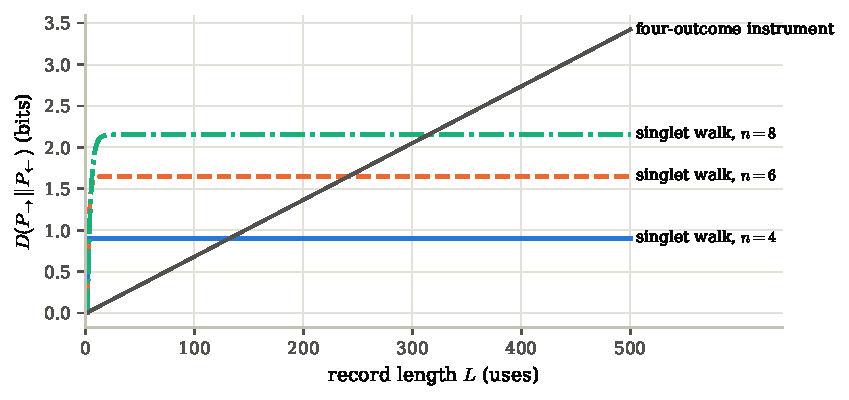
\includegraphics[width=0.9\textwidth]{fig3_arrow.pdf}
\caption{Total irreversibility $D(P_\to\|P_\leftarrow)$ of a record of length $L$. Singlet walks ($n=4,6,8$) saturate at $c\,\mathrm{artanh}(c)/\ln2=0.899,1.645,2.152$ bits, the Jeffreys divergence of their seed pair law from the stationary one. The processed four-outcome instrument of \cref{sec:four} grows linearly, as $(L-1)\,\mathrm{EP}$ with $\mathrm{EP}=0.00686044$ bits per use, and overtakes the $n=4$ total after $132$ uses.}
\label{fig:arrow}
\end{figure}

\paragraph{Values.} For $n=4$, $d=0$ and $\mathcal D_L=0.899124$ bits for every $L\ge3$; for $n=6$, $\mathcal D_L=0.822711,1.234066,\dots,1.645019$ for $L=3,\dots,14$, with limit $1.645421$; for $n=3$, $d<0$ and $\mathcal D_L$ oscillates to its limit $0.396241$. Direct summation over all $2^L$ sequences for $L\le14$ and $n=3,4,5,6,8,16$ agrees with the closed form to $4\times10^{-13}$, and the record law computed from the two-qubit density matrix itself, applying the projectors $P_{X_k}(k\vartheta)$ to the singlet in turn for $n=3,4,5,6,8$ and all $2^8$ sequences of length $8$, agrees with the law of Theorem~1.2 to $6\times10^{-17}$. As $n\to\infty$, $1-c=\frac{\pi^2}{2n^2}+O(n^{-4})$, so $c\,\mathrm{artanh}(c)=\ln\frac{2n}\pi+O(n^{-2}\ln n)$: the limit grows like $\log_2(2n/\pi)$ bits.

\paragraph{What sets the arrow.} By (c) the arrow is a property of the seed: the first two outcomes are correlated ($\rho_0=-c$), the stationary record has uncorrelated adjacent outcomes, and the total irreversibility is exactly the Jeffreys divergence between the two pair laws, realised gradually as the record relaxes at rate $d$ per step. The arrow is independent of entanglement, which is Theorem~1.2(d): the first measurement is of $O(0)=\sigma_z$ on Alice, and after its outcome the singlet is in exactly one of the product states $|0\rangle\otimes|1\rangle$, $|1\rangle\otimes|0\rangle$, with probabilities $\frac12,\frac12$, which is the state the separable preparation is in after the same outcome; every later step acts on these product states in the same way. The density-matrix computation above gives the two record laws equal to $6\times10^{-17}$. What the singlet adds is frame independence: its record law is unchanged by a common rotation of all settings, whereas a separable preparation reproduces it only for the settings it is aligned with. The singlet is the fourth state of $\frac12\otimes\frac12=1\oplus0$, whose triplet $m=-1,0,1$ is the triad \cite{SQuant}; the walk writes its record from that fourth state.

\section{A processed four-outcome instrument: an arrow written continuously}\label{sec:four}
The second instrument is the processed four-outcome instrument of \cite{Singh}: a Bell instrument reconstructed from tomography, with effects $E_a=\sum_re_{ar}|v_{ar}\rangle\langle v_{ar}|$ and conditional output states $\varrho_a=\sum_sq_{as}|w_{as}\rangle\langle w_{as}|$ in spectral form, physically completed by the Kraus family $K_{asr}=\sqrt{e_{ar}q_{as}}\,|w_{as}\rangle\langle v_{ar}|$, with one nonpositive estimate repaired by the maximal positivity factor $0.708418699729814$, and iterated in a common basis. Since $\sum_{s,r}K_{asr}^\dagger K_{asr}=E_a$ and $\sum_{s,r}K_{asr}\varrho K_{asr}^\dagger=\operatorname{Tr}(E_a\varrho)\,\varrho_a$, the instrument is measure-and-prepare: after summing over the unrecorded labels $r,s$ the post-measurement state depends only on the recorded outcome $a$, so the record is a first-order Markov chain, with $C_{ij}=\operatorname{Tr}(E_i\varrho_j)$. Its transition law is
\[
C=\begin{pmatrix}
0.43696297&0.19810609&0.20644079&0.14060033\\
0.16017410&0.46165671&0.13951861&0.22362294\\
0.24443666&0.11892971&0.46061556&0.17659060\\
0.15842628&0.22130750&0.19342504&0.45918613\end{pmatrix}.
\]
We use this eight-digit matrix as given (two of its columns sum to $1.00000001$; renormalising them changes the quantities below by at most one unit in the last digit shown). Everything in this section is a property of this processed instrument. Its stationary law, the normalised eigenvector for eigenvalue $1$, and its spectrum are
\begin{gather*}
\pi=(0.24327934,\,0.24563854,\,0.24991431,\,0.26116781),\\
\operatorname{spec}C=\{1,\,0.35301359,\,0.27498875,\,0.19041903\};
\end{gather*}
the stationary entropy $H(X_t)=H(\pi)=1.9994586$ bits, the entropy rate $h=H(J)-H(\pi)=1.8413629$ bits per use and $I(X_t;X_{t+1})=H(\pi)-h=0.15809572$ bits; the minimal record cost $k_BT_0\ln2\cdot h=1.2763355\,k_BT_0$ per use, for a bath at temperature $T_0$, with the previous record as side information \cite{delRio}; and the centred Poisson potential $\kappa=(0.03023949,-0.02314357,0.00046184,-0.00684277)$, the unique solution of $(I-C^{\mathsf T})\kappa=g-h\mathbf 1$ with $\pi^{\mathsf T}\kappa=0$, where $g_j=-\sum_iC_{ij}\log_2C_{ij}$ is the expected surprisal of a use made from record $j$. (The equation is solvable because $\pi^{\mathsf T}(g-h\mathbf 1)=0$ and the range of $I-C^{\mathsf T}$ is the orthogonal complement of the kernel of $I-C$, which is spanned by $\pi$; its solutions differ by multiples of $\mathbf 1$.) These agree with the values given in \cite{Singh} to the rounding of $C$.

\paragraph{The arrow.} Detailed balance fails ($\max|J-J^{\mathsf T}|=0.00970$) and
\[
\mathrm{EP}=0.00686044\ \text{bits per use}=0.373\%\ \text{of }h .
\]
The four three-cycle affinities are $\mathcal A_{012}=-0.7807$ ($0\to1\to2\to0$), $\mathcal A_{013}=-0.4939$ ($0\to1\to3\to0$), $\mathcal A_{023}=+0.2029$ ($0\to2\to3\to0$) and $\mathcal A_{123}=-0.0840$ ($1\to2\to3\to1$) bits. Only three are independent (the complete graph on four states has three independent cycles): both $\mathcal A_{012}+\mathcal A_{023}$ and $\mathcal A_{013}+\mathcal A_{123}$ equal the four-cycle affinity $-0.5778$. The record circulates round $0\to2\to1\to0$ with odds $2^{0.7807}=1.718:1$ over the reverse. The reversible half $S$ has $h(S)=1.8430756$, so $h(S)-h(C)=\sum_j\pi_j\mathrm{JSD}=0.00171268$, below the bound $\mathrm{EP}/4=0.00171511$ of Theorem~1.1 (ratio $0.99858$), and the four columnwise ratios $\mathrm{JSD}/\mathcal J$ lie between $0.12479$ and $0.12498$, against the ceiling $\frac18$. The odd half is small, $\|A\|_F=0.0418$ against $\|S-\Pi\|_F=0.4882$. For a stationary record of length $L$ the accumulated irreversibility is exactly $(L-1)\,\mathrm{EP}$ (\cref{sec:split}; the stationary boundary terms cancel), which exceeds the total $0.899124$ bits of the $n=4$ singlet walk once $L-1\ge0.899124/0.00686044=131.06$, i.e.\ after $132$ uses (\cref{fig:arrow}). The constant $\frac14$ is sharp (Theorem~1.1(3)): over $2\times10^4$ random chains with $3$ to $6$ states, whose columns are drawn from symmetric Dirichlet laws with parameter uniform on $[0.2,5]$, the largest ratio $(h(S)-h(C))/(\mathrm{EP}/4)$ is $1-1.1\times10^{-10}$ (the $1820$ chains with a columnwise ratio $\mathrm{JSD}/\mathcal J$ above $0.1249$ were evaluated in 60-significant-digit arithmetic).

\paragraph{Fluctuations of the record cost.} Let $f_t=F_{X_{t+1}X_t}$ with $F_{ij}=-\log_2C_{ij}$ be the per-use surprisal, whose stationary mean is $h$ and whose conditional mean given $X_t=j$ is $g_j$. Its stationary variance is $\mathrm{Var}(f_0)=\sum_{ij}J_{ij}(F_{ij}-h)^2=0.46159536$ bits$^2$. For $t\ge1$, $\mathbb E[f_t-h\mid X_1=i]=[(C^{\mathsf T})^{t-1}(g-h\mathbf 1)]_i$, and $\sum_{r\ge0}(C^{\mathsf T})^r(g-h\mathbf 1)=\kappa$ (the series converges geometrically, at the rate $0.353$ of the second eigenvalue, is centred because $\pi^{\mathsf T}C^{\mathsf T}=\pi^{\mathsf T}$, and solves the Poisson equation), so the lagged covariances sum in closed form to
\[
\sum_{t\ge1}\mathrm{Cov}(f_0,f_t)=\sum_{ij}J_{ij}(F_{ij}-h)\,\kappa_i=0.00044146\ \text{bits}^2,
\]
and the Markov central limit theorem \cite{MeynTweedie} gives
\[
\sigma^2=\mathrm{Var}(f_0)+2\sum_{t\ge1}\mathrm{Cov}(f_0,f_t)=0.46247828\ \text{bits}^2\ \text{per use}.
\]
The empirical rate after $N$ uses therefore lies in $h\pm1.96\sigma/\sqrt N=h\pm1.333/\sqrt N$ bits with 95\% probability (to leading order in $N$). Beside this there is a deterministic bias: for a record started at $x_0$, $g-h\mathbf 1=\kappa-C^{\mathsf T}\kappa$ gives $\mathbb E[g_{X_t}]-h=\mathbb E[\kappa_{X_t}]-\mathbb E[\kappa_{X_{t+1}}]$, so $\mathbb E\sum_{t<N}(f_t-h)=\kappa_{x_0}-\mathbb E[\kappa_{X_N}]$, and the bias of the rate is at most $2\max_j|\kappa_j|/N=0.0605/N$ bits \cite{Singh}. Under an accounting that charges each record its surprisal, the cost of $N$ uses has mean $1.2763355\,N\,k_BT_0$ and standard deviation $0.680\ln2\sqrt N=0.471\sqrt N\,k_BT_0$; Landauer's principle bounds the heat of erasing the record from below by the mean \cite{Landauer,ReebWolf,delRio}. The total-variation distance of the law of $X_t$ to $\pi$, maximised over the initial record (the largest half column-sum of $|C^t-\Pi|$), is $0.216$, $0.069$, $3.2\times10^{-3}$, $1.8\times10^{-5}$ after $t=1,2,5,10$ uses (spectral gap $1-0.353=0.647$).

\section{The same involution in a rotating field}\label{sec:field}
Three coils at angles $0,\pm120^\circ$ carrying alternating currents produce, in complex notation, the rotating field $B(t)$ of Theorem~1.3 \cite{Ferraris,Tesla}. We identify $B=B_x+iB_y$ with the column vector $(B_x,B_y)^{\mathsf T}$, and now prove Theorem~1.3.
\begin{proof}[Proof of Theorem~1.3]
$i_k=\frac12(I_k\e^{i\omega t}+\bar I_k\e^{-i\omega t})$, $I_a+uI_b+u^{-1}I_c=3I_+$ and $\bar I_a+u\bar I_b+u^{-1}\bar I_c=\overline{I_a+u^{-1}I_b+uI_c}=3\overline{I_-}$, which gives the form of $B$. (1) Since $1+u+u^{-1}=0$, adding a common $I_0$ to all three currents changes nothing. Exchanging $I_b$ and $I_c$ exchanges the definitions of $I_+$ and $I_-$. $B(-t)=\alpha_+\e^{-i\omega t}+\alpha_-\e^{i\omega t}$, whose forward and backward amplitudes are $|\alpha_-|$ and $|\alpha_+|$. (2) $\bar B\dot B=i\omega\bigl(|\alpha_+|^2-|\alpha_-|^2+z-\bar z\bigr)$ with $z=\bar\alpha_-\alpha_+\e^{2i\omega t}$, and $i\omega(z-\bar z)$ is real, so $B_x\dot B_y-B_y\dot B_x=\Im(\bar B\dot B)=\omega(|\alpha_+|^2-|\alpha_-|^2)$ is constant, and over a period $2\pi/\omega$ the signed area $\frac12\oint(B_x\,dB_y-B_y\,dB_x)=\pi(|\alpha_+|^2-|\alpha_-|^2)$. The sum of two counter-rotating circular motions is an ellipse with semi-axes $|\alpha_+|+|\alpha_-|$ and $\bigl||\alpha_+|-|\alpha_-|\bigr|$. (3) For the reversed field $B_r(t)=B(-t)$, the substitution $t'=-t-\tau$, under which the period average is invariant, gives $\langle B_r(t+\tau)B_r(t)^{\mathsf T}\rangle=\langle B(t')B(t'+\tau)^{\mathsf T}\rangle=K(\tau)^{\mathsf T}$. Next, $\langle\bar B(t)B(t+\tau)\rangle=|\alpha_+|^2\e^{i\omega\tau}+|\alpha_-|^2\e^{-i\omega\tau}$, because the cross terms carry $\e^{\pm2i\omega t}$ and average to zero. Its real part is $\langle B_x(t)B_x(t+\tau)+B_y(t)B_y(t+\tau)\rangle=\operatorname{tr}K(\tau)$ and its imaginary part is $\langle B_x(t)B_y(t+\tau)-B_y(t)B_x(t+\tau)\rangle=K_{yx}(\tau)-K_{xy}(\tau)$. (4) The antisymmetric part of a $2\times2$ matrix is fixed by $K_{yx}-K_{xy}$, which by (3) vanishes for every $\tau$ iff $\Phi=0$, i.e.\ iff $|I_+|=|I_-|$. If $|\alpha_+|=|\alpha_-|=r$ and $\alpha_\pm=r\e^{i\theta_\pm}$, then $B(t)=2r\,\e^{i(\theta_++\theta_-)/2}\cos\bigl(\omega t+\frac{\theta_+-\theta_-}2\bigr)$, a linear oscillation symmetric about $t_0=-(\theta_+-\theta_-)/2\omega$. Conversely, if $B(t_0+t)=B(t_0-t)$, then $B_x\dot B_y-B_y\dot B_x$ changes sign under $t\mapsto2t_0-t$; being constant, it is zero, and $\Phi=0$.
\end{proof}
A single coil gives $|I_+|=|I_-|=\frac13|I_a|$: its field pulsates with zero swept area. A balanced set in one order is pure forward rotation (area $\frac{9\pi}4|I|^2=7.0686$ for $|I|=1$), in the other pure backward rotation. For the unbalanced example $(1,\,0.8\angle{-120^\circ},\,1.1\angle{118^\circ})$ the forward and backward amplitudes $|\alpha_+|$ and $|\alpha_-|$ are $1.4498$ and $0.1203$ and the swept area is $\Phi=+6.5578$. The decomposition is Fortescue's method of symmetrical components \cite{Fortescue,Clarke}.

\paragraph{The shared structure.} Theorems~1.1 and~1.3 are two instances of one structure. A stationary process $W_t$ with values in $\R^m$ has lagged correlation matrices $K(\tau)=\mathbb E[W_{t+\tau}W_t^{\mathsf T}]$, and time reversal acts on them by transposition, $K(\tau)\mapsto K(\tau)^{\mathsf T}=K(-\tau)$. For the record, $W_t=e_{X_t}$ is the indicator vector of the outcome and $K(1)=J$, so time reversal is $J\mapsto J^{\mathsf T}$, that is $C\mapsto\tilde C$; for the field, $W_t=B(t)$. In both, the symmetric half carries magnitude: $S$, the reversible chain with the same $\pi$ and the larger entropy rate; and $\operatorname{tr}K(0)=|\alpha_+|^2+|\alpha_-|^2$, the mean-square field. In both, the antisymmetric half carries a signed circulation: the cycle currents $J-J^{\mathsf T}=2AD_\pi$, which vanish exactly when every cycle affinity does; and the swept area $\Phi$, through $K_{yx}-K_{xy}=(\Phi/\pi)\sin\omega\tau$. In both, the antisymmetric half vanishes exactly on the reversible set: $J=J^{\mathsf T}$ (detailed balance, every affinity zero), and $|I_+|=|I_-|$ (the field is a linear oscillation, reversible about $t_0$). The two differ in how distance from the reversible set is measured: EP is a divergence of $J$ from $J^{\mathsf T}$ and is nonnegative, whereas $\Phi$ is linear in the antisymmetric half and carries its sign, as the cycle currents do.

\section{Three bodies: exact statements}\label{sec:exact}
Throughout \cref{sec:exact,sec:eight,sec:contrast,sec:fourth} the model is the planar Newtonian problem in dimensionless units, $G=1$, with unit masses for the triad; positions are $x_i\in\R^2$, or $z_i\in\C$ in complex notation, and $\mathcal L=\sum_im_i\,x_i\times\dot x_i$ is the angular momentum. We prove the four parts of Theorem~1.4 in turn. Part (a) is a statement about the centre of mass.
\begin{proof}[Proof of Theorem~1.4(a)]
$x_a+x_b=2x_m$ and $x_a+x_b+x_m=0$ give $3x_m=0$, and then $x_a=-x_b$.
\end{proof}
The middle body is the zero of the pair $\pm s$, at the pair's centre \cite{SZero}. Part (b) is a statement about Fourier coefficients.
\begin{proof}[Proof of Theorem~1.4(b)]
$\sum_iz_i(t)=\sum_k\hat q_k\e^{2\pi ikt/T}(1+u^{\nu k}+u^{2\nu k})$ with $u=\e^{2\pi i/3}$. The bracket is $3$ if $3\mid k$ and $0$ otherwise, so $\sum_i z_i\equiv0$ forces $\hat q_k=0$ for $3\mid k$, by uniqueness of Fourier coefficients. $\Im(\bar z\dot z)$ is a unit mass's angular momentum. Since $\dot q=\sum_k(2\pi ik/T)\hat q_k\e^{2\pi ikt/T}$, Parseval's identity gives the period average $\langle\bar q\dot q\rangle=(2\pi i/T)\sum_kk|\hat q_k|^2$, so each body, whose path is a time shift of $q$, has average angular momentum $(2\pi/T)\sum_kk|\hat q_k|^2$. The total $\mathcal L$ is constant, hence equal to its average, three times this.
\end{proof}
The phases $1,u,\bar u$ are the triad of the circle: the pair $u,\bar u$ sums to $-1$ and balances the third. The centre of mass sees only the harmonics in which this balance fails, and these must vanish. The same identity $1+u+u^2=0$ removes the common mode $I_0$ from the field of Theorem~1.3, which is built from the phases $1,u,u^{-1}$ of the three coils. Part (c) rests on a symmetry of Newton's equations.
\begin{proof}[Proof of Theorem~1.4(c)]
For equal masses, Newton's equations $\ddot x_i=\sum_{j\ne i}(x_j-x_i)/|x_j-x_i|^3$ are invariant under $(t,x_1,x_2,x_3)\mapsto(-t,-x_2,-x_1,-x_3)$. Indeed, write $F_i(x)=\sum_{j\ne i}(x_j-x_i)/|x_j-x_i|^3$ and $y_1(t)=-x_2(-t)$, $y_2(t)=-x_1(-t)$, $y_3(t)=-x_3(-t)$. Then $\ddot y_1(t)=-\ddot x_2(-t)=-F_2(x(-t))$, and $F_1(y(t))=-F_2(x(-t))$ because $y_2-y_1=-(x_1-x_2)$ and $y_3-y_1=-(x_3-x_2)$ at time $-t$; bodies 2 and 3 are alike. Each velocity changes sign twice, so the map sends $\dot x_1(0)$ to $\dot x_2(0)=\dot x_1(0)$ and $\dot x_3(0)$ to itself, and it sends $x_1(0)$ to $-x_2(0)=x_1(0)$ and $x_3(0)=0$ to itself; it therefore fixes the initial data. By uniqueness the solution equals its image. Body 3's path $z_3(t)=\sum_k\hat z_k\e^{2\pi ikt/T}$, with $\hat z_k=u^{2\nu k}\hat q_k$, is odd, so $\hat z_{-k}=-\hat z_k$ and $|\hat q_{-k}|=|\hat z_{-k}|=|\hat z_k|=|\hat q_k|$. In $\mathcal L=(6\pi/T)\sum_kk|\hat q_k|^2$ the terms $k|\hat q_k|^2$ and $-k|\hat q_{-k}|^2$ cancel in pairs.
\end{proof}
The body at the zero has a past that is the negative of its future: a pair in time. The map of the proof sends $x_i\times\dot x_i$ to $-x_{i'}\times\dot x_{i'}$ with $i'$ the partner label, so it reverses $\mathcal L$; a solution fixed by it has $\mathcal L=0$, exactly as a record fixed by time reversal has no cycle current.

\paragraph{The Lagrange triangle.} Three masses at the vertices of an equilateral triangle rotating rigidly at angular velocity $\omega$ form the Lagrange relative equilibrium. With $M=\sum_im_i$ and $\beta=\sum_{i<j}m_im_j/M^2$, its nontrivial linear exponents solve $\lambda^4+\omega^2\lambda^2+\tfrac{27}{4}\beta\,\omega^4=0$, so $\lambda^2=\omega^2\bigl(-1\pm\sqrt{1-27\beta}\bigr)/2$. The motion is linearly stable exactly when these are real, negative and distinct, that is when $27\sum_{i<j}m_im_j<M^2$ (Gascheau \cite{Gascheau}, Routh \cite{Routh}). At the boundary $27\beta=1$ the two imaginary pairs meet at $\pm i\omega/\sqrt2$, and beyond it they leave the imaginary axis as a quadruple $\{\lambda,-\lambda,\bar\lambda,-\bar\lambda\}$. For a star, a planet of mass fraction $\mu$ and a test body, $\beta=\mu(1-\mu)$ and the criterion reads $\mu<\mu_G=(1-\sqrt{23/27})/2=0.0385209$; this is the stability of the triangular points $L_4,L_5$, satisfied by all four giant planets, whose Trojans are treated in \cite{SPlanet}. For equal masses, $27\sum_{i<j}m_im_j=81>9=M^2$ and $\beta=\tfrac13$, so $\lambda^2=\omega^2(-1\pm i\sqrt8)/2$ and
$\lambda=\omega(\pm1/\sqrt2\pm i)$, since $(1/\sqrt2+i)^2=-\tfrac12+i\sqrt2$. The growth rate is
\begin{equation}\label{eq:routh}
\max\Re\lambda=\omega/\sqrt2 .
\end{equation}
We derive this directly for unit masses, which proves Theorem~1.4(d).
\begin{proof}[Proof of Theorem~1.4(d)]
In complex coordinates rotating at $\omega$, $z_j=\e^{i\omega t}w_j$, Newton's equations read $\ddot w_j+2i\omega\dot w_j-\omega^2w_j=\sum_{k\ne j}f(w_k-w_j)$ with $f(v)=v/|v|^3$. The triangle $w_j=Ru^j$ of side $a=\sqrt3R$ is an equilibrium: $\sum_{k\ne j}(w_k-w_j)/a^3=-3w_j/a^3$, so $\omega^2=3/a^3$. Since $\partial f/\partial v=-\tfrac12|v|^{-3}$ and $\partial f/\partial\bar v=-\tfrac32\hat v^2|v|^{-3}$ with $\hat v=v/|v|$, a perturbation $w_j=Ru^j+\chi_j$ obeys
\[
\ddot\chi_j+2i\omega\dot\chi_j-\omega^2\chi_j=-\frac1{2a^3}\sum_{k\ne j}(\chi_k-\chi_j)-\frac3{2a^3}\sum_{k\ne j}\hat v_{jk}^2(\bar\chi_k-\bar\chi_j),
\]
where $\hat v_{j,j\pm1}^2=u^{2j}\e^{\mp i\pi/3}$. For $\chi_j=u^{2j}b(t)$ the first sum is $-3u^{2j}b$, and the second is $u^{3j}\bigl[\e^{-i\pi/3}(u-1)+\e^{i\pi/3}(u^{-1}-1)\bigr]\bar b=(i\sqrt3-i\sqrt3)\bar b=0$. So this mode decouples and $\ddot b+2i\omega\dot b-\tfrac32\omega^2b=0$; with $b=\e^{\lambda t}$, $\lambda^2+2i\omega\lambda-\tfrac32\omega^2=0$, $\lambda=\omega(-i\pm1/\sqrt2)$, and the real form of this complex equation adds the conjugates: $\lambda=\omega(\pm1/\sqrt2\pm i)$, the roots of the quartic at $\beta=\tfrac13$. The remaining modes, $\chi_j$ the same for all $j$ (translations) and $\chi_j=u^jb_1(t)$ (rotation and dilation of the triangle), have only the exponents $0$ and $\pm i\omega$.
\end{proof}
The eigenvalues of the Jacobian of the equations of motion in the rotating frame, formed by central differences with step $10^{-6}$, give $\max\Re\lambda/\omega=0.707106781$.

\section{The figure-eight: one curve, thirds of the period, six triads}\label{sec:eight}
All orbits are integrated in double precision with the explicit Runge--Kutta method of order 8 of Dormand and Prince with adaptive step size and continuous (dense) output, DOP853 \cite{HNW}, applied to $\ddot x_i=\sum_{j\ne i}m_j(x_j-x_i)/|x_j-x_i|^3$, here with relative and absolute tolerance $10^{-13}$. For the published data $\mathcal L(0)=x_1\times\dot x_1+x_2\times\dot x_2=x_1\times\dot x_1-x_1\times\dot x_1=0$ exactly, and, since $\dot x_1=\dot x_2=-\dot x_3/2$ and the mutual distances are $2|x_1|,|x_1|,|x_1|$, the energy is $E=\tfrac34|\dot x_3|^2-5/(2|x_1|)=-1.287141991766$.

\paragraph{Period.} Minimising the distance $|\mathrm{state}(t)-\mathrm{state}(0)|$ in $\R^{12}$ (positions and velocities) over $t\in[6.2,6.45]$, using the dense output and bounded Brent minimisation, gives $T=6.3259140121$ with return residual $1.6\times10^{-9}$. This agrees with the published $6.32591398$ to $3.2\times10^{-8}$, the rounding level of eight-digit data; at tolerance $10^{-11}$, $T$ moves by $4.6\times10^{-10}$.

\paragraph{Choreography.} With the labels of the published data, the three bodies follow one curve with
\[
x_{i+1}(t)=x_i(t-T/3)=x_i(t+2T/3)\qquad(\text{indices mod }3),
\]
to $1.3\times10^{-8}$ (maximum over $2001$ equally spaced $t\in[0,T]$ and over $i$), which is Theorem~1.4(b) with $\nu=-1$.

\paragraph{Refined data.} Keeping the positions and $\dot x_1=\dot x_2=-\dot x_3/2$, and solving for $\dot x_3$ and $T$ by Levenberg--Marquardt least squares on the twelve components of $\mathrm{state}(T)-\mathrm{state}(0)$, gives $\dot x_3=(-0.932407368139,-0.864731461835)$, $T=6.325914009781$, residual $9.6\times10^{-13}$. The change in $\dot x_3$ is $2.6\times10^{-9}$, so the published digits are right to their last place; the choreography then holds to $4.1\times10^{-12}$.

\paragraph{Six triads per period.} The signed area $\Delta(t)=\tfrac12(x_2-x_1)\times(x_3-x_1)$ of the triangle of the bodies, sampled at $6001$ points of $(-T/12,T-T/12]$ with its sign changes refined by bracketing root-finding, vanishes exactly six times per period. The zeros lie at $kT/6$ to $5.5\times10^{-9}$. At each one the middle body lies at the midpoint to $4.8\times10^{-9}$ and at the centre of mass to $3.2\times10^{-9}$, as Theorem~1.4(a) requires. The middle bodies are $3,2,1,3,2,1$ in turn: each body holds the zero twice per period. The half-length $|s|$ is the same at all six to $1.7\times10^{-9}$; at $t=0$ it is $|x_1(0)|=(0.97000436^2+0.24308753^2)^{1/2}=1.0000000028$. The axis alternates between $165.9312^\circ$ (at $t=0$, $180^\circ-\arctan(0.24308753/0.97000436)$) and $14.0688^\circ$: as point sets there are only two triads, $\{-s,0,s\}$ and its mirror image, each visited three times with the roles passed round the bodies (\cref{fig:main}a).

\paragraph{Accuracy of the integration.} Sampling every $T/64$, over one period the relative energy error is at most $6.9\times10^{-13}$ and $|\mathcal L|\le1.7\times10^{-12}$. Over 50 periods the bounds are $2.7\times10^{-11}$ and $2.4\times10^{-12}$.

\paragraph{Harmonics.} Over one refined period we take the discrete Fourier coefficients $\hat q_k=\frac1{4096}\sum_{n=0}^{4095}z_1(nT/4096)\e^{-2\pi ikn/4096}$ of $z_1=x_1+iy_1$. Those with $3\mid k$, $|k|\le60$, are at most $7.2\times10^{-13}$ of the largest (Theorem~1.4(b)). The largest are $|\hat q_{\pm1}|=0.5504$, $|\hat q_{\pm2}|=0.1694$, $|\hat q_{\pm4}|=0.02798$ and $|\hat q_{\pm5}|=0.01270$; even harmonics are present. On the computed orbit $\max_t|x_3(-t)+x_3(t)|=2.9\times10^{-12}$ and $\max_k\bigl||\hat q_k|-|\hat q_{-k}|\bigr|/\max|\hat q|=3.8\times10^{-13}$, as Theorem~1.4(c) requires; the power $\sum|\hat q_k|^2$ is $0.332616$ in $k>0$ and in $k<0$, and $(6\pi/T)\sum k|\hat q_k|^2=5.7\times10^{-13}$: the eight is a sum of balanced counter-rotating pairs of circles.

\begin{figure}[t]\centering
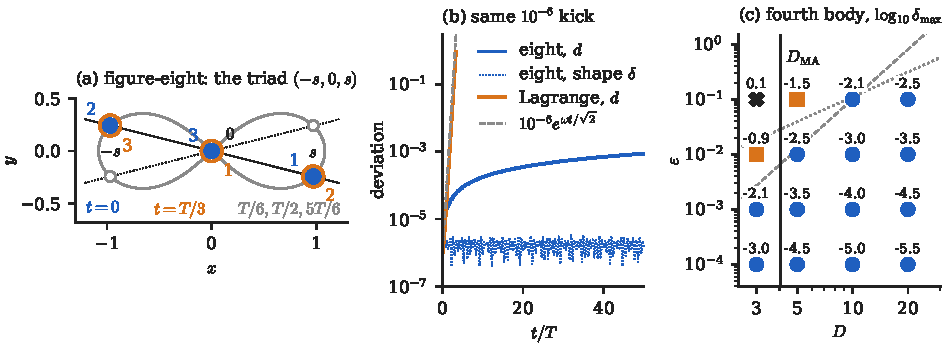
\includegraphics[width=\linewidth]{fig_phys2.pdf}
\caption{(a) The eight (grey). At $t=0$ (blue, labels $1,2,3$) the bodies are at $s,-s,0$; at $t=T/3$ (orange rings) they occupy the same points with body $1$ at the zero. Open circles: the mirror triad at $T/6,T/2,5T/6$. (b) Deviation after the same $10^{-6}$ kick: for the eight, the equal-time distance $d_{\mathrm{eq}}$ and the shape deviation $\delta$; for the Lagrange triangle, $d_{\mathrm{eq}}$ (stopped at $1$), with the rate \eqref{eq:routh} dashed. (c) $\log_{10}\delta_{\max}$ over $100\,T$ for a fourth body of mass $\varepsilon$ at distance $D$: kept (blue), deformed (orange), broken (black; value before break-up). Dashed: $\varepsilon/D^3=10^{-4}$; dotted: $\delta_{\max}=10^{-2}$ from \eqref{eq:law}; vertical: the Mardling--Aarseth distance $D_{\mathrm{MA}}$.}\label{fig:main}
\end{figure}

\section{A triad in motion against a triangle at rest}\label{sec:contrast}
The Lagrange triangle gets the same period, $\omega=2\pi/T=0.9932454496$, with side $a=(3/\omega^2)^{1/3}=1.4487808456$ from $\omega^2=3/a^3$ (\cref{sec:exact}), and both orbits the same kick, $+10^{-6}$ to $x$ of body~1. $d_{\mathrm{eq}}(t)$ is the equal-time distance in $\R^6$ to the unperturbed orbit (for Lagrange, the exact rotation), sampled every $T/64$ on $[0,50T]$; $\delta(t)$ is the shape deviation of \cref{sec:fourth}. The Lagrange integration stops when $d_{\mathrm{eq}}$ reaches $1$.

The figure-eight's $d_{\mathrm{eq}}$ grows linearly: $1.70\times10^{-5}$ at $T$, $1.72\times10^{-4}$ at $10T$ and $8.57\times10^{-4}$ at $50T$. Its maximum is $8.9\times10^{-4}$, and the least-squares slope of $\log\max_{r\le t}d_{\mathrm{eq}}(r)$ against $\log t$ over $[5T,50T]$ is $1.003$. This is drift along the family's neutral directions (phase, orientation); its shape stays within $3.2\times10^{-6}$ of the eight. The Lagrange $d_{\mathrm{eq}}$ passes $0.1$ at $2.875\,T$ and $1$ at $3.389\,T$, and its shape deviation reaches $0.87$. Its rate, the least-squares slope of $\log d_{\mathrm{eq}}$ against $t$ from the first time $d_{\mathrm{eq}}\ge10^{-5}$ to the first time $d_{\mathrm{eq}}>10^{-2}$, is $0.702194$, against $\omega/\sqrt2=0.702331$, a difference of $0.02\%$.

We repeated the comparison for eight random kicks of norm $10^{-6}$, with independent standard normal components in $\R^6$, the centre-of-mass part removed and the result rescaled to norm $10^{-6}$. The Lagrange $d_{\mathrm{eq}}$ passes $0.1$ after every one of them, with fitted rates $0.63197$--$0.70224$. The figure-eight's shape stays within $5.3\times10^{-6}$, and its equal-time distance reaches at most $1.68\times10^{-3}$; the growth is phase drift, linear in time and in the energy change.

\section{A fourth body}\label{sec:fourth}
\paragraph{Set-up and measure.} A body of mass $\varepsilon$ starts at distance $D$ from the centre of mass of the refined eight, in direction $+x$, with circular two-body relative speed $\sqrt{(3+\varepsilon)/D}$ in direction $+y$, in the barycentric frame (the triad is shifted by $-\varepsilon/(3+\varepsilon)$ and the fourth body by $3/(3+\varepsilon)$ of the relative position and velocity), so that $3X_{\mathrm{triad}}+\varepsilon x_4=0$. The grid is $\varepsilon\in\{10^{-4},10^{-3},10^{-2},10^{-1}\}$, $D\in\{3,5,10,20\}$, with integrations over $100\,T$ at tolerance $10^{-12}$, sampled every $T/64$. With $Y(t)$ the triad positions about the triad's own centre of mass and $Y_8(\tau)$ the same for one period of the eight,
\[
\delta(t)=\min_{\tau\in[0,T),\ \theta}\ \bigl\|Y(t)-R_\theta Y_8(\tau)\bigr\|_F ,
\]
with $R_\theta$ the rotation by $\theta$. For fixed $\tau$ the minimum over rotations is closed-form: $\min_\theta\|Y-R_\theta Z\|_F^2=\|Y\|_F^2+\|Z\|_F^2-2\bigl(\langle Y,Z\rangle^2+(\sum_iZ_i\times Y_i)^2\bigr)^{1/2}$, because $\langle Y,R_\theta Z\rangle=\cos\theta\,\langle Y,Z\rangle+\sin\theta\sum_iZ_i\times Y_i$. $Y_8$ is interpolated by a periodic cubic spline through $4096$ samples of one period, and $\tau$ is found on a $2048$-point grid followed by golden-section refinement (a $20001$-point scan with Brent refinement gives the same $\delta$ to $3.6\times10^{-10}$). A case is \emph{kept} if all inner distances stay below $3$ and $\delta_{\max}<10^{-2}$, \emph{deformed} if they stay below $3$ but $\delta_{\max}\ge10^{-2}$, and \emph{broken} otherwise (the integration stops when an inner distance reaches $3$). We write $\eta=\varepsilon/D^3$ for the tidal parameter.

\begin{table}[t]\centering\small
\begin{tabular}{@{}r cccc c@{}}\toprule
 & \multicolumn{4}{c}{$\delta_{\max}$ over $100\,T$ for $\varepsilon=$} & outer orbit\\
$D$ & $10^{-4}$ & $10^{-3}$ & $10^{-2}$ & $10^{-1}$ & ($P_{\mathrm{out}}/T$; fate)\\\midrule
3 & $9.26\times10^{-4}$ & $7.45\times10^{-3}$ & $0.132^{\,d}$ & $1.21^{\,b}$ & 2.980; expelled in all four\\
5 & $3.27\times10^{-5}$ & $3.26\times10^{-4}$ & $3.20\times10^{-3}$ & $0.0315^{\,d}$ & 6.411; bound, $r/D\in[0.893,1]$\\
10 & $9.30\times10^{-6}$ & $9.29\times10^{-5}$ & $9.22\times10^{-4}$ & $8.33\times10^{-3}$ & 18.134; bound\\
20 & $3.19\times10^{-6}$ & $3.18\times10^{-5}$ & $3.145\times10^{-4}$ & $2.87\times10^{-3}$ & 51.291; bound\\\bottomrule
\end{tabular}
\caption{Stability map of the triad with a fourth body; $d$ deformed, $b$ broken (at $15.43\,T$), others kept. $P_{\mathrm{out}}=2\pi\sqrt{D^3/3}$. Control $\varepsilon=0$: floor $5.2\times10^{-8}$.}\label{tab:map}
\end{table}

\paragraph{The map (\cref{tab:map}, \cref{fig:main}c).} All 15 cases with $\eta<10^{-3}$ survive. At fixed $D$, $\delta_{\max}$ is linear in $\varepsilon$: among kept cases with $\varepsilon\le10^{-2}$, $\delta_{\max}/\varepsilon$ varies by at most a factor $1.244$ at $D=3$ and $1.021$ for $D\ge5$. In $\eta$ the grid splits cleanly: every case with $\eta\le10^{-4}$ is kept and every case with $\eta\ge3.7\times10^{-4}$ is not, so the threshold lies in $(10^{-4},3.7\times10^{-4})$: $(D,\varepsilon)=(5,0.1)$ and $(3,0.01)$ are deformed and $(3,0.1)$ breaks. Over the kept cases $\delta_{\max}/\eta$ ranges from $40.0$ to $254.8$, growing with $D$ for $D\ge5$: the tidal parameter alone does not set the deformation. The next paragraph identifies what does.

\paragraph{What sets it: the spin the fourth body lends and takes back.} Let $Y_i=(\xi_i,\zeta_i)$ be the triad positions about its centre of mass ($\sum_iY_i=0$, unit masses) and let the fourth body be at distance $D$ in direction $\hat R=(\cos\psi,\sin\psi)$, $\psi=\Omega t$, $\Omega=\sqrt{(3+\varepsilon)/D^3}$. Expanding the potential energy $-\sum_i\varepsilon/|D\hat R-Y_i|$ to second order in $|Y_i|/D$, the monopole term drives the outer orbit, the dipole term cancels because $\sum_iY_i=0$, and the quadrupole term is
\[
V=-\frac{\varepsilon}{2D^3}\sum_i\bigl[3(\hat R\cdot Y_i)^2-|Y_i|^2\bigr]=-\frac{3\varepsilon}{2D^3}\Bigl[\tfrac12\Delta I\cos2\psi+I_{xy}\sin2\psi\Bigr]+\text{const},
\]
with $I_{xx}=\sum\xi_i^2$, $I_{yy}=\sum\zeta_i^2$, $I_{xy}=\sum\xi_i\zeta_i$ and $\Delta I=I_{xx}-I_{yy}$, the constant not depending on $\psi$. Rotating the triad by $\phi$ changes $\psi$ to $\psi-\phi$, so the torque on it is $\Gamma=-\partial V/\partial\phi=\partial V/\partial\psi=(3\varepsilon/2D^3)(\Delta I\sin2\psi-2I_{xy}\cos2\psi)$. Averaged over the inner period, with $\langle I_{xy}\rangle=3.8\times10^{-9}$ and $\langle\Delta I\rangle=1.641896$ (means over $4096$ equally spaced samples of one period of the refined eight, which is elongated along $x$), this is $\Gamma=(3\varepsilon/2D^3)\langle\Delta I\rangle\sin2\Omega t$. Integrating from $\mathcal L_{\mathrm{in}}(0)=0$ gives the triad a spin
\[
\mathcal L_{\mathrm{in}}(t)=\frac{3\varepsilon\langle\Delta I\rangle}{4\Omega D^3}\,(1-\cos2\Omega t),\qquad \max_t\mathcal L_{\mathrm{in}}=\frac{3\varepsilon\langle\Delta I\rangle}{2\Omega D^3}.
\]
The torque is a pair: it is odd under $t\mapsto\pi/\Omega-t$, so over each half outer orbit its positive and negative halves cancel, and the spin returns to zero. In integrations at $\varepsilon=10^{-3}$, $D\in\{5,7,10,14,20,28\}$, the measured $\max|\mathcal L_{\mathrm{in}}|$, with $\mathcal L_{\mathrm{in}}=\sum_iY_i\times\dot Y_i$ about the triad's centre of mass, exceeds this maximum by the ratios $1.1361$ ($D=5$), $1.0244$ ($D=10$) and $1.0030$ ($D=28$); the measured ratio $\delta_{\max}/\max|\mathcal L_{\mathrm{in}}|$ tends to $1.985$; and the least-squares slopes against $\log D$ for $D\ge10$ are $-1.535$ ($\log\delta_{\max}$) and $-1.520$ ($\log\max|\mathcal L_{\mathrm{in}}|$), against $-\tfrac32$ from the formula. Combining the measured $\delta_{\max}\simeq2\max|\mathcal L_{\mathrm{in}}|$ with $\max\mathcal L_{\mathrm{in}}$ and $\Omega\simeq\sqrt3D^{-3/2}$ for $\varepsilon\ll3$ gives, at leading order,
\begin{equation}\label{eq:law}
\delta_{\max}\simeq2\max|\mathcal L_{\mathrm{in}}|\simeq\sqrt3\,\langle\Delta I\rangle\,\varepsilon D^{-3/2}=2.8438\,\varepsilon D^{-3/2}.
\end{equation}
Across the grid of \cref{tab:map}, $\delta_{\max}$ equals \eqref{eq:law} times $1.24$--$1.28$ ($D=5$), $0.93$--$1.03$ ($D=10$) and $0.90$--$1.00$ ($D=20$). The governing parameter is $\varepsilon D^{-3/2}\propto(\varepsilon/D^3)\,P_{\mathrm{out}}$, the tidal strength times the time over which it acts coherently. By \eqref{eq:law}, $\delta_{\max}=10^{-2}$ at $\varepsilon D^{-3/2}=10^{-2}/2.8438=3.516\times10^{-3}$, which in terms of $\eta=(\varepsilon D^{-3/2})D^{-3/2}$ is $3.15\times10^{-4}$ at $D=5$, $1.11\times10^{-4}$ at $D=10$ and $3.93\times10^{-5}$ at $D=20$. The deformation is reversible: at $D=20$, $\varepsilon=10^{-3}$, where half an outer period is $\pi/\Omega=25.641\,T$, the minimum of $\delta$ within $1.5\,T$ of each of the first three half outer periods is $5.96\times10^{-8}$, $4.22\times10^{-8}$ and $6.66\times10^{-8}$, the $\varepsilon=0$ floor, against $\delta_{\max}=3.18\times10^{-5}$. At tolerance $10^{-13}$, $\delta_{\max}$ is $3.150319\times10^{-2}$ at $(5,0.1)$ (unchanged) and $0.1325148$ at $(3,0.01)$ (against $0.1324405$ at $10^{-12}$); the chaotic case $(3,0.1)$ breaks at $10.71\,T$ (against $15.43\,T$).

\paragraph{The new pair and the Mardling--Aarseth boundary.} For a circular coplanar prograde outer orbit, Mardling and Aarseth's stability criterion for hierarchical triples \cite{MA} is $D>2.8\,a_{\mathrm{in}}(1+q_{\mathrm{out}})^{2/5}$, $q_{\mathrm{out}}=\varepsilon/3$ the outer-to-inner mass ratio. With $a_{\mathrm{in}}=(3(T/2\pi)^2)^{1/3}=1.448781$ (by Kepler's third law, the semi-major axis of a binary of mass $3$ and period $T$, equal to the side $a$ of the Lagrange triangle of \cref{sec:contrast}), $D_{\mathrm{MA}}=4.0566$--$4.1101$ over the four values of $\varepsilon$. At $D=3$, inside the boundary, the fourth body is expelled in every case, ending at $r/D=83.2$, $47.5$, $401.7$, $85.1$ with positive two-body energy. At $D\ge5$ the $3+1$ pair stays bound, though not exactly circular: at $D=5$, $r/D\in[0.893,1.000]$, an excursion of up to $0.1065$. The same excursion occurs at $\varepsilon=0$: it is the triad's own quadrupole acting on a point-mass circular start, and it falls to $0.0238$--$0.0258$ at $D=10$ and $0.0059$--$0.0062$ at $D=20$. Energy is conserved to $1.1\times10^{-9}$ in the surviving cases and to $5.2\times10^{-7}$ in the broken case, and at tolerance $10^{-13}$ to $9.8\times10^{-11}$ and $2.7\times10^{-9}$. The complementary limit, a third body of vanishing mass near one member of a pair, is Hill's problem, whose two throats at $L_1$ and $L_2$ are treated in \cite{SPlanet}.

\paragraph{The fourth element.} The figure-eight is the triad in motion, with the zero passing round the bodies; the rigid triangle, with no body at the zero, is unstable. The fourth body and the triad form a new pair about their joint centre, $3X_{\mathrm{triad}}+\varepsilon x_4=0$, a triad seen from outside: outside the Mardling--Aarseth boundary it lends the triad a spin and takes it back every half outer orbit; inside it the new pair does not form.

\section{Discussion: one involution across records, fields and orbits}\label{sec:one}
Each system of this paper carries an involution $\iota$, a map equal to its own inverse. Every quantity $Q$ splits into an even half $\frac12(Q+\iota Q)$ and an odd half $\frac12(Q-\iota Q)$, and an odd quantity vanishes on every object that $\iota$ fixes. \Cref{tab:involution} lists the six instances; each entry is proved or computed in the section cited.

\begin{table}[!htb]\centering\small
\begin{tabular}{@{}>{\raggedright\arraybackslash}p{2.8cm}>{\raggedright\arraybackslash}p{4.1cm}>{\raggedright\arraybackslash}p{3.0cm}>{\raggedright\arraybackslash}p{4.7cm}@{}}\toprule
System & Involution $\iota$ & Odd quantity & On the fixed set; computed value\\\midrule
Measurement record, \S\S\ref{sec:split},~\ref{sec:four} & time reversal, $J\mapsto J^{\mathsf T}$ & cycle currents $J-J^{\mathsf T}$ & zero iff detailed balance; four-outcome instrument: $\max|J-J^{\mathsf T}|=0.00970$\\
Singlet walk, \S\ref{sec:singlet} & sequence reversal & $\log(P_\to/P_\leftarrow)$ & zero for the stationary record; total $c\,\mathrm{artanh}(c)$ nats from the seed\\
Three-phase field, \S\ref{sec:field} & $K(\tau)\mapsto K(\tau)^{\mathsf T}$; $b\leftrightarrow c$ & swept area $\Phi$ & zero iff $|I_+|=|I_-|$; example $\Phi=6.5578$\\
Figure-eight, \S\S\ref{sec:exact},~\ref{sec:eight} & $(t,x_1,x_2,x_3)\mapsto$ $(-t,-x_2,-x_1,-x_3)$ & angular momentum $\mathcal L$ & zero harmonic by harmonic; computed $5.7\times10^{-13}$\\
Lagrange triangle, \S\S\ref{sec:exact},~\ref{sec:contrast} & $\lambda\mapsto-\bar\lambda$ on the spectrum & $\Re\lambda$ & zero iff $27\sum m_im_j\le M^2$ (stable iff $<$); equal masses $\pm\omega/\sqrt2$, computed $0.702194$\\
Fourth body, \S\ref{sec:fourth} & $t\mapsto\pi/\Omega-t$ & averaged torque $\Gamma$ & spin returns to zero each half outer orbit; $\delta$ returns to the $5\times10^{-8}$ floor\\\bottomrule
\end{tabular}
\caption{One involution, six instances. In each, the odd half vanishes on the set fixed by $\iota$.}\label{tab:involution}
\end{table}

Three structural points connect the two halves of the paper.

\emph{The pair.} In the record, the reversible half $S$ and the odd half $A$ are the even and odd parts of $C$ under time reversal, and Theorem~1.1 measures the cost of the odd half: it can take from the entropy rate at most one quarter of what it produces, and for the four-outcome instrument it takes within $0.15\%$ of that quarter. In the field, the forward and backward components $\alpha_\pm$ are exchanged by the same involution, and the swept area is their signed difference. In the figure-eight, the harmonics $\hat q_k$ and $\hat q_{-k}$ are counter-rotating circles of equal radius, paired by the time-reversal symmetry, and the angular momentum, their signed difference, vanishes.

\emph{The triad.} The phases $1,u,\bar u$ of the three coils, of the three bodies at thirds of the period, and of the vertices of the Lagrange triangle are the same triad of the circle, with $1+u+\bar u=0$. In the field the identity removes the common mode $I_0$; in the choreography it removes every harmonic divisible by three; in the Lagrange triangle it decouples the mode $\chi_j=u^{2j}b$ that carries the instability. The same identity makes a probe qubit coupled to a maximally mixed spin-1 decohere completely at $\frac13$ and $\frac23$ of its revival period \cite{SQuant}. Among three equal masses, the triad with a body at the zero, the figure-eight, is linearly stable \cite{Roberts} and keeps its shape to $3.2\times10^{-6}$ after a kick, while the rigid triangle, with no body at the zero, leaves at $\omega/\sqrt2$; and a triangle of general masses stands only around a dominant centre: since $\sum_{i<j}m_im_j=m_1(M-m_1)+m_2m_3\ge m_1(M-m_1)$ for the largest mass $m_1$, the criterion $27\sum_{i<j}m_im_j<M^2$ forces $27x(1-x)<1$ with $x=m_1/M$, that is $x<\mu_G$ or $x>1-\mu_G$, and $x\ge\frac13>\mu_G$ leaves $m_1>(1-\mu_G)M=0.9614791\,M$ \cite{Gascheau,Routh,SPlanet}.

\emph{The fourth element.} The observer writes the record; the stationary singlet record, written from the fourth state of $\frac12\otimes\frac12$, is reversible, and its whole arrow is the seed correlation. The fourth body, watching the triad from outside, forms a new pair with it, $3X_{\mathrm{triad}}+\varepsilon x_4=0$, and its effect on the triad is itself a pair in time: the spin lent over one quarter of the outer orbit is returned over the next.

\paragraph{Outlook.} With the raw tomographic counts behind the matrix $C$ of \cref{sec:four}, the sampling uncertainty of its entropy production, $\mathrm{EP}=0.00686$ bits per use, can be computed and set against it. The next step for the fourth body is to carry the quadrupole torque of \cref{sec:fourth} to eccentric and inclined outer orbits.

\section{Data and sources}\label{sec:data}
No observational dataset is used. The external inputs are the following.
\begin{itemize}
\item \emph{Transition matrix of the processed four-outcome instrument} (\cref{sec:four}): the $4\times4$ column-stochastic matrix $C$ displayed there, to eight decimal places, is taken from \cite{Singh}, \S9, Eq.~(24) (repeated in its App.~E, Eq.~(50)), together with the maximal positivity factor $0.708418699729814$ (\cite{Singh}, \S8, Eq.~(23)). In \cite{Singh}, $C$ is obtained from processed, publicly available tomographic estimates of a four-outcome Bell-measurement instrument (effects $E_a$ and conditional output states $\varrho_a$), physically completed by the Kraus family $K_{asr}$ and expressed in a common basis; that source gives no raw counts or covariance and does not identify the underlying measurement further. Only the matrix $C$ is used here; every quantity in \cref{sec:four} and \cref{fig:arrow} is computed from it. The values of $\pi$, $\operatorname{spec}C$, $H(X_t)$, $h$, $I(X_t;X_{t+1})$, $\kappa$ and the bias bound given in \cite{Singh}, \S\S9--11, agree with ours to the rounding of $C$.
\item \emph{Singlet walk} (\cref{sec:singlet}): no external data; all numbers follow from the closed forms of Theorem~1.2, with $c=\cos(\pi/n)$, $d=\cos(2\pi/n)$.
\item \emph{Random chains} (\cref{sec:four}): drawn as described there; no external dataset.
\item \emph{Rotating field} (\cref{sec:field}): the currents $(1,\,0.8\angle{-120^\circ},\,1.1\angle{118^\circ})$ are an illustrative choice.
\item \emph{Initial data of the figure-eight} (computed by Sim\'o and published by Chenciner and Montgomery \cite{CM}): $x_1=-x_2=(0.97000436,-0.24308753)$, $x_3=(0,0)$, $\dot x_3=-2\dot x_1=-2\dot x_2=(-0.93240737,-0.86473146)$, published period $6.32591398$. The refined data of \cref{sec:eight} are derived from these.
\item \emph{Lagrange triangle}: the characteristic quartic and the stability criterion of Gascheau and Routh \cite{Gascheau,Routh}, derived in \cref{sec:exact} for unit masses.
\item \emph{Mardling--Aarseth criterion} \cite{MA}: constant $2.8$ and exponent $2/5$, used with outer eccentricity $0$ and zero mutual inclination.
\item \emph{Integration method}: the order-8 Dormand--Prince pair with dense output, DOP853 \cite{HNW}.
\item \emph{Stability of the eight} (context, no numbers taken): Roberts \cite{Roberts}; numerical studies by Sim\'o \cite{Simo}; discovery by Moore \cite{Moore}.
\item \emph{Physical constants}: none enter numerically. The three-body problem is in dimensionless units, $G=1$; record costs are stated in units of $k_BT_0$.
\end{itemize}
All other parameters (kicks, $\varepsilon$, $D$, tolerances, sampling steps, grid sizes, numbers of settings) are choices stated where they are used.

\paragraph{Contributions and use of AI.} The ideas, the research questions, the framework that links the fields, the choice of problems and the direction at every stage are the author's. The derivations, proofs, numerical checks, reference checks and drafting were produced with an AI system working under that direction, and were checked by separate AI review passes. Errors in that material are errors of the AI system, and any found will be corrected in a revised version. Publication-ethics policy (COPE, \emph{Authorship and AI tools}, 2023) does not allow an AI system to be listed as an author, so its use is declared here instead.

\begin{thebibliography}{99}\small\setlength{\itemsep}{1pt}\setlength{\parskip}{0pt}
\bibitem{Bell} J.~S.~Bell, On the Einstein Podolsky Rosen paradox, \emph{Physics Physique Fizika} 1 (1964) 195--200.
\bibitem{CM} A.~Chenciner, R.~Montgomery, A remarkable periodic solution of the three-body problem in the case of equal masses, \emph{Ann. of Math.} 152 (2000) 881--901.
\bibitem{Clarke} E.~Clarke, \emph{Circuit Analysis of A-C Power Systems}, Vol.~I, Wiley, New York, 1943.
\bibitem{delRio} L.~del Rio, J.~\AA berg, R.~Renner, O.~Dahlsten, V.~Vedral, The thermodynamic meaning of negative entropy, \emph{Nature} 474 (2011) 61--63.
\bibitem{Dressel} J.~Dressel, A.~Chantasri, A.~N.~Jordan, A.~N.~Korotkov, Arrow of time for continuous quantum measurement, \emph{Phys. Rev. Lett.} 119 (2017) 220507.
\bibitem{Ferraris} G.~Ferraris, Rotazioni elettrodinamiche prodotte per mezzo di correnti alternate, \emph{Il Nuovo Cimento} 23 (1888) 246--263.
\bibitem{Fill} J.~A.~Fill, Eigenvalue bounds on convergence to stationarity for nonreversible Markov chains, with an application to the exclusion process, \emph{Ann. Appl. Probab.} 1 (1991) 62--87.
\bibitem{Fortescue} C.~L.~Fortescue, Method of symmetrical co-ordinates applied to the solution of polyphase networks, \emph{Trans. AIEE} 37 (1918) 1027--1140.
\bibitem{Gascheau} G.~Gascheau, Examen d'une classe d'\'equations diff\'erentielles et applications \`a un cas particulier du probl\`eme des trois corps, \emph{C. R. Acad. Sci. Paris} 16 (1843) 393.
\bibitem{Gaspard} P.~Gaspard, Time-reversed dynamical entropy and irreversibility in Markovian random processes, \emph{J. Stat. Phys.} 117 (2004) 599--615.
\bibitem{GaspardErr} P.~Gaspard, Erratum: Time-reversed dynamical entropy and irreversibility in Markovian random processes, \emph{J. Stat. Phys.} 126 (2007) 1109.
\bibitem{HNW} E.~Hairer, S.~P.~N{\o}rsett, G.~Wanner, \emph{Solving Ordinary Differential Equations I: Nonstiff Problems}, 2nd ed., Springer, Berlin, 1993.
\bibitem{KPV} R.~Kawai, J.~M.~R.~Parrondo, C.~Van den Broeck, Dissipation: the phase-space perspective, \emph{Phys. Rev. Lett.} 98 (2007) 080602.
\bibitem{KS} S.~Kochen, E.~P.~Specker, The problem of hidden variables in quantum mechanics, \emph{J. Math. Mech.} 17 (1967) 59--87.
\bibitem{Kraus} K.~Kraus, \emph{States, Effects, and Operations}, Lecture Notes in Physics 190, Springer, Berlin, 1983.
\bibitem{Landauer} R.~Landauer, Irreversibility and heat generation in the computing process, \emph{IBM J. Res. Dev.} 5 (1961) 183--191.
\bibitem{MA} R.~A.~Mardling, S.~J.~Aarseth, Tidal interactions in star cluster simulations, \emph{Mon. Not. R. Astron. Soc.} 321 (2001) 398--420.
\bibitem{MeynTweedie} S.~P.~Meyn, R.~L.~Tweedie, \emph{Markov Chains and Stochastic Stability}, 2nd ed., Cambridge University Press, Cambridge, 2009.
\bibitem{Moore} C.~Moore, Braids in classical dynamics, \emph{Phys. Rev. Lett.} 70 (1993) 3675--3679.
\bibitem{ReebWolf} D.~Reeb, M.~M.~Wolf, An improved Landauer principle with finite-size corrections, \emph{New J. Phys.} 16 (2014) 103011.
\bibitem{Roberts} G.~E.~Roberts, Linear stability analysis of the figure-eight orbit in the three-body problem, \emph{Ergodic Theory Dynam. Systems} 27 (2007) 1947--1963.
\bibitem{RoldanParrondo} \'E.~Rold\'an, J.~M.~R.~Parrondo, Estimating dissipation from single stationary trajectories, \emph{Phys. Rev. Lett.} 105 (2010) 150607.
\bibitem{Routh} E.~J.~Routh, On Laplace's three particles, with a supplement on the stability of steady motion, \emph{Proc. London Math. Soc.} 6 (1874) 86--97.
\bibitem{Schnakenberg} J.~Schnakenberg, Network theory of microscopic and macroscopic behavior of master equation systems, \emph{Rev. Mod. Phys.} 48 (1976) 571--585.
\bibitem{Simo} C.~Sim\'o, Dynamical properties of the figure eight solution of the three-body problem, in \emph{Celestial Mechanics (Evanston, IL, 1999)}, Contemp. Math. 292, Amer. Math. Soc., Providence, RI, 2002, 209--228.
\bibitem{Singh} A.~Singh, Sequential quantum instruments: depletion, regeneration, and minimal predictive state, preprint, August 2026.
\bibitem{SQuant} A.~Singh, The Riemann Kernel as a Quantum State: Wigner Negativity, Decoherence at the Thirds and Lee--Yang Zeros, manuscript, 25 September 2026.
\bibitem{SPlanet} A.~Singh, The Four Giants as Balanced Pairs: Throats, Hearts, the Gas Ladder and the Interstellar Visitors, manuscript, 25 September 2026.
\bibitem{SZero} A.~Singh, What a Zero Is: One Involution across Mathematics, Physics, Chemistry, Neuroscience, Computation and the Giant Planets, manuscript, 25 September 2026.
\bibitem{Tesla} N.~Tesla, Electro-magnetic motor, U.S. Patent 381,968, issued 1 May 1888.
\end{thebibliography}
\end{document}
